\documentclass{article}
\usepackage[T2A]{fontenc}
\usepackage[utf8]{inputenc}
\usepackage[english, ukrainian]{babel}
\usepackage{graphicx}
\graphicspath{ {images/} }
\usepackage{float}
\usepackage{multicol}
\usepackage{blindtext}

\title{Лабораторна робота 3.
	
Розв’язування задач на обчислення за допомогою Excel.
}
\author{Автор, вчитель інформатики Гулич Андрій Васильович}

\begin{document}
	
	\maketitle
	\subsection*{\textit{Тема: Ровв'язування задач на обчислення. }}
	\subsection*{\textit{Мета: Навчитись використовувати Excel для розв'язування елементарних завдань. }} 
	
	\subsection*{\textit{Цілі: }} 
	\begin{enumerate}
		\item Закріпити навики з використання абсолютних, відносних та мішаних величин
		\item Повторити навики роботи з рядком формул та автозаповненням
	\end{enumerate}
	\begin{center}
	\subsection*{\textit{Хід роботи: }} 
	\subsection*{\textbf{Завдання 1. Степені натуральних чисел. }} 
	\end{center}

	Засобами табличного процесора створіть електронну таблицю степенів натуральних чисел першого десятка від першого степеня до п'ятого.
	
	\begin{enumerate}
		\item Відкрийте програму Excel . Створіть таблицю.
		\begin{center}
			\begin{tabular}{|p{0.03\textwidth} | p{0.1\textwidth}|p{0.1\textwidth}|p{0.1\textwidth}|p{0.1\textwidth}|p{0.1\textwidth}|p{0.1\textwidth}|}
				\hline
				 & A & B & C & D & E & F \\ 
				\hline
				1 & \multicolumn{6}{|c|}{В степені} \\
				\hline
				2 & Число & 1 & 2 & 3 & 4 & 5 \\
				\hline
				3 & 1 &  &  &  &  &  \\
				\hline
				4 & 2 &  &  &  &  &  \\
				\hline
				5 & 3 &  &  &  &  &  \\
				\hline
				6 & 4 &  &  &  &  &  \\
				\hline
				7 & 5 &  &  &  &  &  \\
				\hline
				8 & 6 &  &  &  &  &  \\
				\hline
				9 & 7 &  &  &  &  &  \\
				\hline
				10 & 8 &  &  &  &  &  \\
				\hline
				11 & 9 &  &  &  &  &  \\
				\hline
				12 & 10 &  &  &  &  &  \\
				\hline
			\end{tabular}
		\end{center}
		\item 2.	Для клітинки В3 уведіть формулу =A3*\$B\$2 (при цьому зроблене абсолютне посилання на клітинку В2, тобто перший степінь) і протягніть автозаповненням для всіх клітинок стовпця В (В4:В12). Аналогічно зробіть для інших стовпців.
		
		\item Ви отримаєте ось таку таблицю:
		\begin{center}
			\begin{tabular}{|p{0.03\textwidth} | p{0.1\textwidth}|p{0.1\textwidth}|p{0.1\textwidth}|p{0.1\textwidth}|p{0.1\textwidth}|p{0.1\textwidth}|}
				\hline
				& A & B & C & D & E & F \\ 
				\hline
				1 & \multicolumn{6}{|c|}{В степені} \\
				\hline
				2 & Число & 1 & 2 & 3 & 4 & 5 \\
				\hline
				3 & 1 & 1 & 1 & 1 & 1 & 1 \\
				\hline
				4 & 2 & 2 & 4 & 8 & 16 & 32 \\
				\hline
				5 & 3 & 3 & 9 & 27 & 81 & 243 \\
				\hline
				6 & 4 & 4 & 16 & 64 & 256 & 1024 \\
				\hline
				7 & 5 & 5 & 25 & 125 & 625 & 3125 \\
				\hline
				8 & 6 & 6 & 36 & 216 & 1296 & 7776 \\
				\hline
				9 & 7 & 7 & 49 & 343 & 2401 & 16807 \\
				\hline
				10 & 8 & 8 & 64 & 512 & 4096 & 32768 \\
				\hline
				11 & 9 & 9 & 81 & 729 & 6561 & 59049 \\
				\hline
				12 & 10 & 10 & 100 & 1000 & 10000 & 100000 \\
				\hline
			\end{tabular}
		\end{center}
	\end{enumerate}
	
	\begin{center}
		\subsection*{\textbf{Завдання 2. Об'єм газу. }}
	\end{center}

	Засобами табличного процесора створіть електронну таблицю для визначення об'єму газу за нормальних умов.
	\begin{enumerate}
		\item Відкрийте програму Excel . Створіть таблицю.
		\begin{figure}[h]
			\centering
			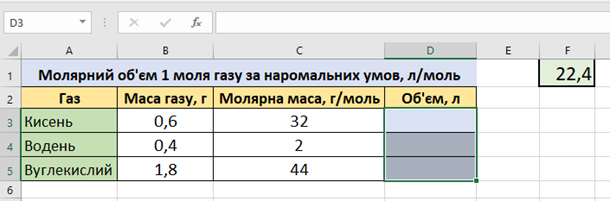
\includegraphics[width=0.8\linewidth]{Excel1.png}
		\end{figure}
		\item Для визначення об’єму газу користуються формулою: 
		В клітинку D3 введіть формулу: =B3/C3*\$F\$1, де  \$F\$1 це  абсолютне посилання на клітинку.
		\item Скопіюйте дану формулу автоматично для клітинок D4:D5.
		\newpage
		\item Отримаємо таблицю:
		\begin{figure}[h]
			\centering
			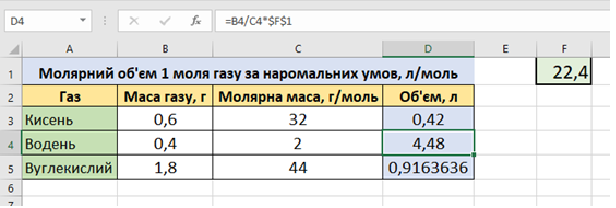
\includegraphics[width=0.8\linewidth]{Excel2.png}
		\end{figure}
	\end{enumerate}
	\subsection*{\textbf{Висновки: }}
\end{document}